\chapter{Sigue personas}
\label{cap:capitulo5}
Ahora que ya tenemos integrado ROS2 dentro de la plataforma de VisualCircuit, vamos a crear varios proyectos usando los bloques drivers que hemos creado. El primero de ellos será un comportamiento de \textit{follow-person} usando reconocimiento visual.

\section{Desarrollo inicial sigue-personas}
\label{sec:VC_intro}

En primer lugar, debemos preparar el entorno de pruebas, por lo que aprovecharemos un modelo de persona teleoperada que creó Carlos Caminero\footnote{\url{https://github.com/RoboticsLabURJC/2021-tfg-carlos-caminero/tree/main/amazon_hospital/hospital_world}}, compañero de la carrera.

\begin{figure} [H]
    \begin{center}
        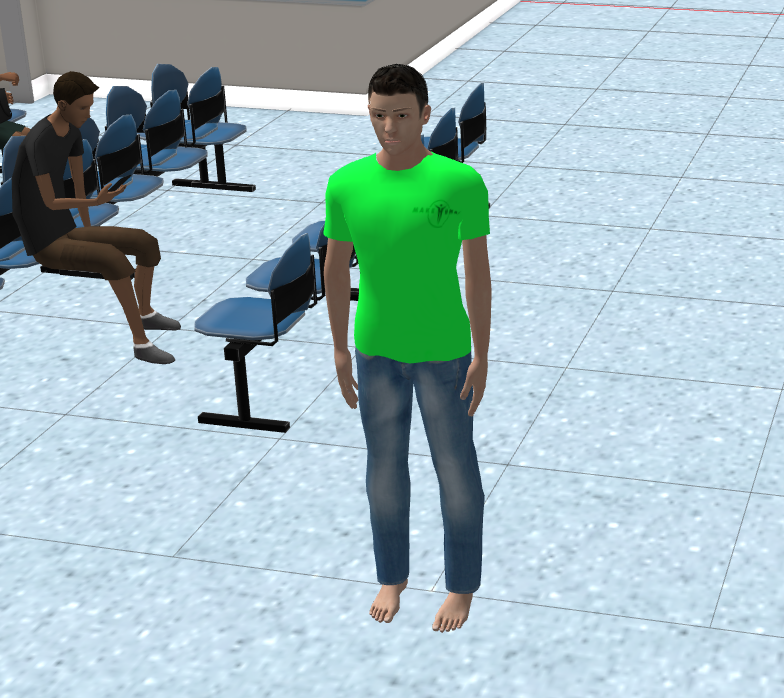
\includegraphics[width=8cm]{figs/c5/elman.png}
    \end{center}
    \caption[Modelo de persona en gazebo]{Modelo de persona teleoperable en gazebo.}
    \label{fig:teleop_person}
\end{figure}

El mundo que tenía Carlos creado incluía muchos elementos del entorno que no son necesarios en nuestro caso, por lo que modificaremos el mundo para dejar únicamente al robot y a la persona. El modelo del robot que usaremos será el que mencionamos en el capítulo \ref{subsec:turtlebot2_sim}, ya que incluye tanto cámara como láser.\\

Para desarrollar el comportamiento sigue-persona con VisualCircuit, 





















